\chapter{Results}
\label{cha:results}

\section{Graphene on Ir}

The quality of the graphene was checked each time D$_2$ was dosed on the sample, in order to ensure that the amount of defects was at a minimum. STM pictures of pure graphene on Ir(111) is shown in this section. On figure \ref{GrIr} pictures of graphene on Ir in different sizes is shown. Figure \ref{GrIr1} shows a large image of a graphene monolayer covering the Ir surface. Although the quality of the image is of low quality, the moire pattern is perceived. Also several step edges from the underlying Ir surface is seen. Several line scans has been performed on these edges, which show that the height difference is 2Å $\pm$0.4Å. This value is consistent with the value of 0.22nm found in the litterature.\cite{1367-2630-11-2-023006}\\
On figure \ref{GrIr2} a high resolution image of Gr/Ir is seen. The moire pattern is very prominent in this figure, and the spacing between the individual sites in the moire unit cell can be determined from a line scan. A line scan was drawn on figure \ref{GrIr2} and two points were positioned in the corners of the moire unit cell in order to obtain the moire periodicity. The morié periodicity is 25.2 $\pm$ 0.4Å according to the litterature.\cite{1367-2630-10-4-043033} This agrees with the measured length of 25.24 Å from the line scan. Typical defects on of the graphene monolayer is seen as well in this figure. Also the hexagonal pattern of graphene is sensed because of the atomic resolution. On figure \ref{GrIr3} the individual carbon atoms are even more clear.\\

\begin{figure}[H]
\makebox[\textwidth][c]{
  \begin{subfigure}[b]{0.3\paperwidth}
    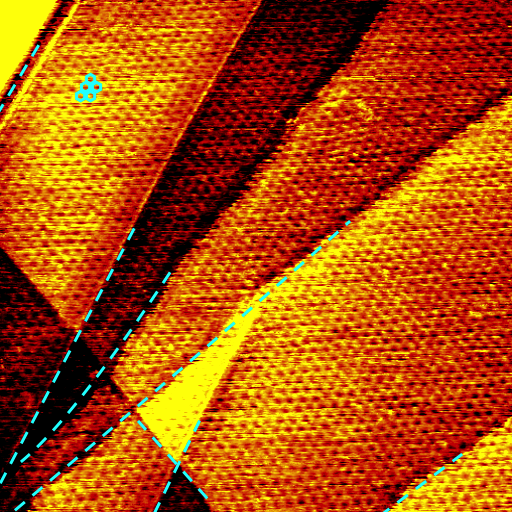
\includegraphics[height=\textwidth]{STMdata/FFT/2016-04-11_000_33.png}
    \caption{993x993 Å - 0.690 nA 78.1 mV}
    \label{GrIr1}
  \end{subfigure}
  \begin{subfigure}[b]{0.3\paperwidth}
    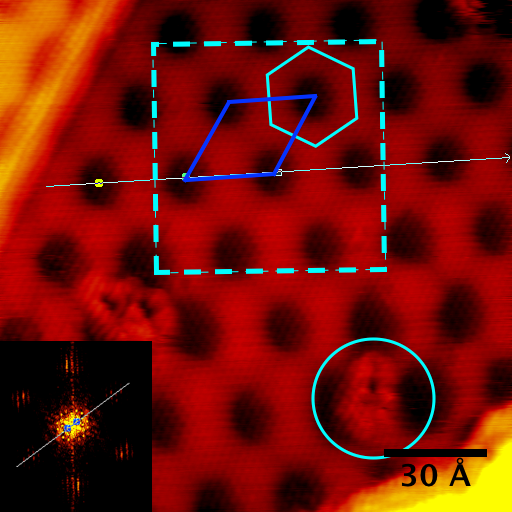
\includegraphics[height=\textwidth]{STMdata/FFT/2016-04-11_000_50.png}
    \caption{148x148 Å - -0.890 nA -311.3 mV}
    \label{GrIr2}
  \end{subfigure}
  \begin{subfigure}[b]{0.3\paperwidth}
    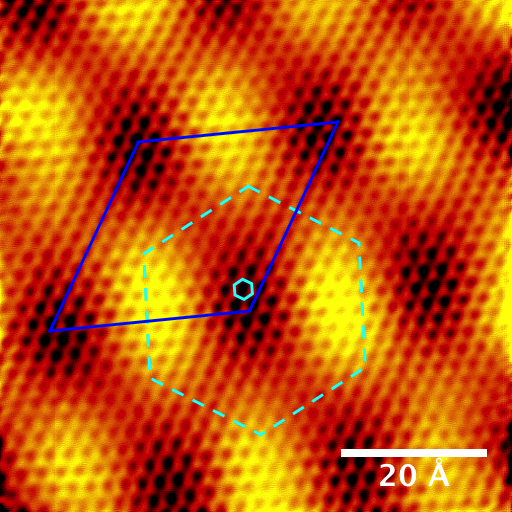
\includegraphics[height=\textwidth]{STMdata/FFT/2016-04-11_000_56.png}
    \caption{70x70 Å - 0.910 nA 311.3 mV}
    \label{GrIr3}
  \end{subfigure}
}
\caption{}
\label{GrIr}
\end{figure}

\section{D2 on graphene}

Dosing at temperatures of, 1340C, 1540C and 1740C were performed in order to determine the threshold temperature of the hydrogenation of graphene.

Full coverage D2 on graphene




1740 C doser ...

\begin{figure}[H]
\makebox[\textwidth][c]{
  \begin{subfigure}[b]{0.3\paperwidth}
    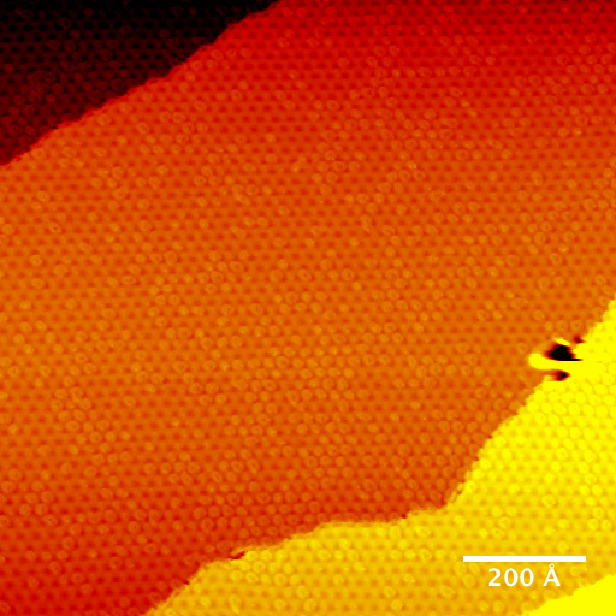
\includegraphics[height=\textwidth]{STMdata/FFT/2016-04-11_003_14.png}
    \caption{998x998 Å - 1060 nA 67.1 mV}
    \label{}
  \end{subfigure}
  \begin{subfigure}[b]{0.3\paperwidth}
    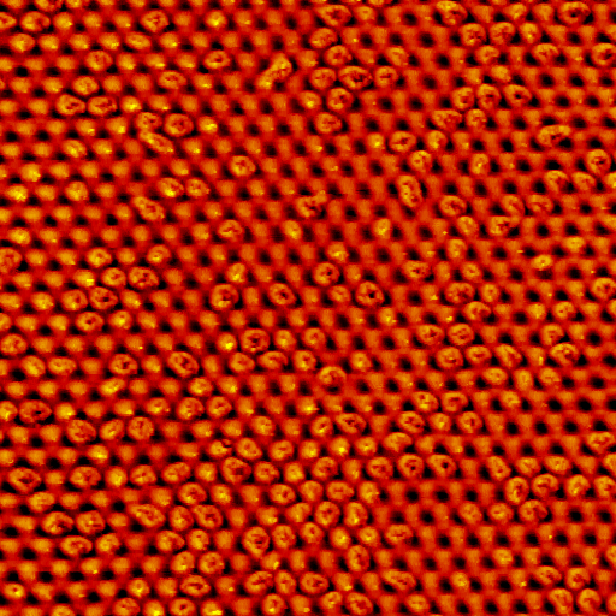
\includegraphics[height=\textwidth]{STMdata/FFT/2016-04-11_003_15.png}
    \caption{497x497 Å - 1.080 nA 67.1 mV}
    \label{}
  \end{subfigure}
  \begin{subfigure}[b]{0.3\paperwidth}
    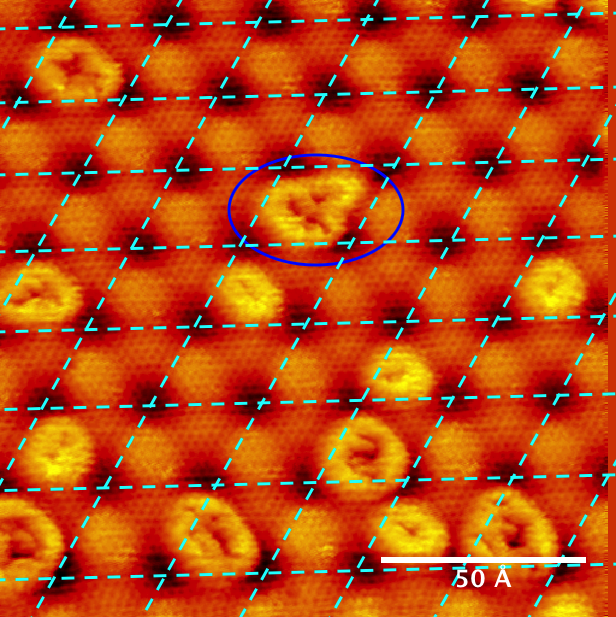
\includegraphics[height=\textwidth]{STMdata/FFT/2016-04-11_003_23.png}
    \caption{150x150 Å - 1.090 nA 67.1 mV}
    \label{}
  \end{subfigure}
}
\caption{}
\label{}
\end{figure}

1593 C doser ...

\begin{figure}[H]
\makebox[\textwidth][c]{
  \begin{subfigure}[b]{0.3\paperwidth}
    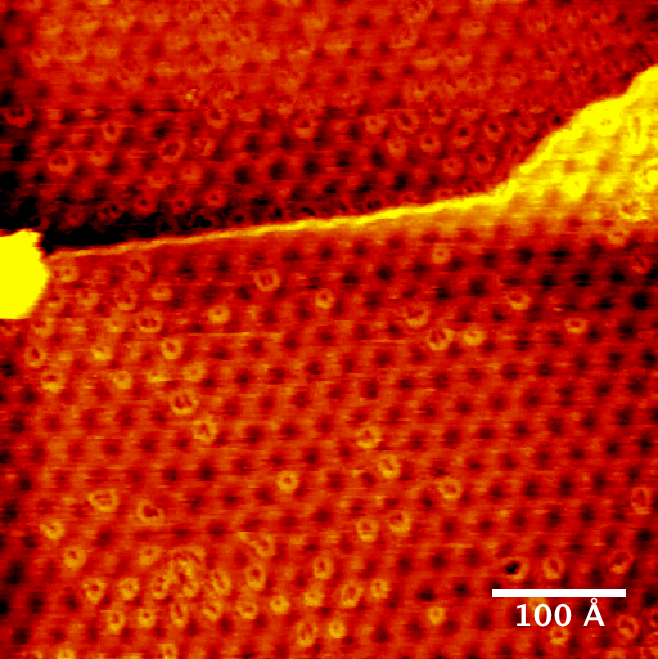
\includegraphics[height=\textwidth]{STMdata/FFT/2016-04-14_000_44.png}
    \caption{488x488 Å - 0.900 nA 190.4 mV}
    \label{}
  \end{subfigure}
  \begin{subfigure}[b]{0.3\paperwidth}
    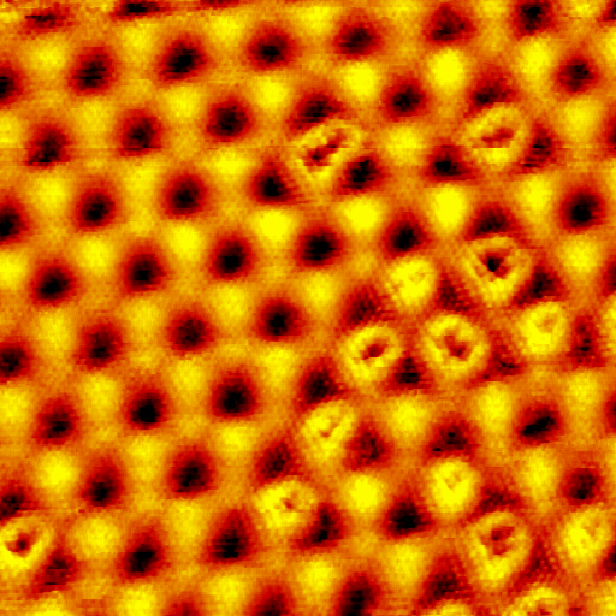
\includegraphics[height=\textwidth]{STMdata/FFT/2016-04-14_000_27.png}
    \caption{180x180Å - 1.020 nA 190.4 mV}
    \label{}
  \end{subfigure}
  \begin{subfigure}[b]{0.3\paperwidth}
    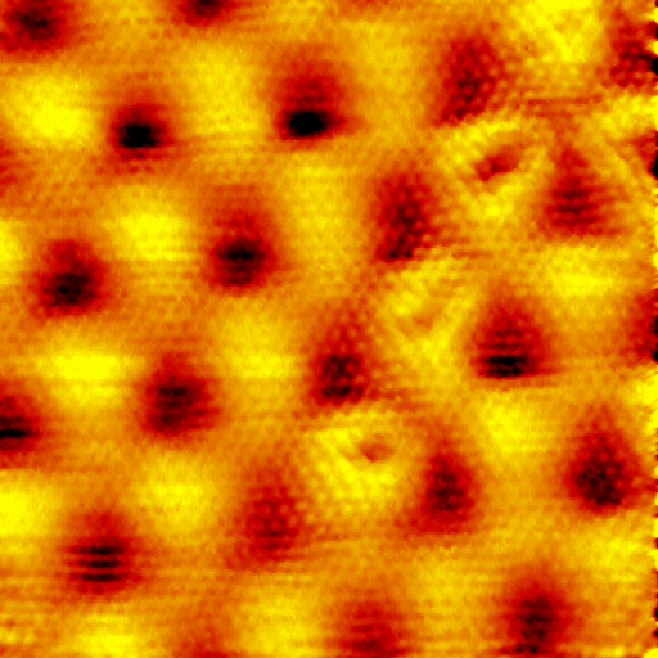
\includegraphics[height=\textwidth]{STMdata/FFT/2016-04-14_000_29.png}
    \caption{97x97 Å - 1020nA, 190.4mV}
    \label{}
  \end{subfigure}
}
\caption{}
\label{}
\end{figure}



\section{TPD measurements - Atomic and molecular D2}

In figure \ref{TPD:all} below, the data from the TPD is gathered in two different figures. TPD measurements were made for both the vibrationally excited molecules and atoms. Figure \ref{TPD:D2} shows the data aquired for the D2 dose and figure \ref{TPD:D} shows the data for the dose with hot atoms.

\begin{figure}[H]
  \centering
  \begin{subfigure}[b]{0.45\textwidth}
    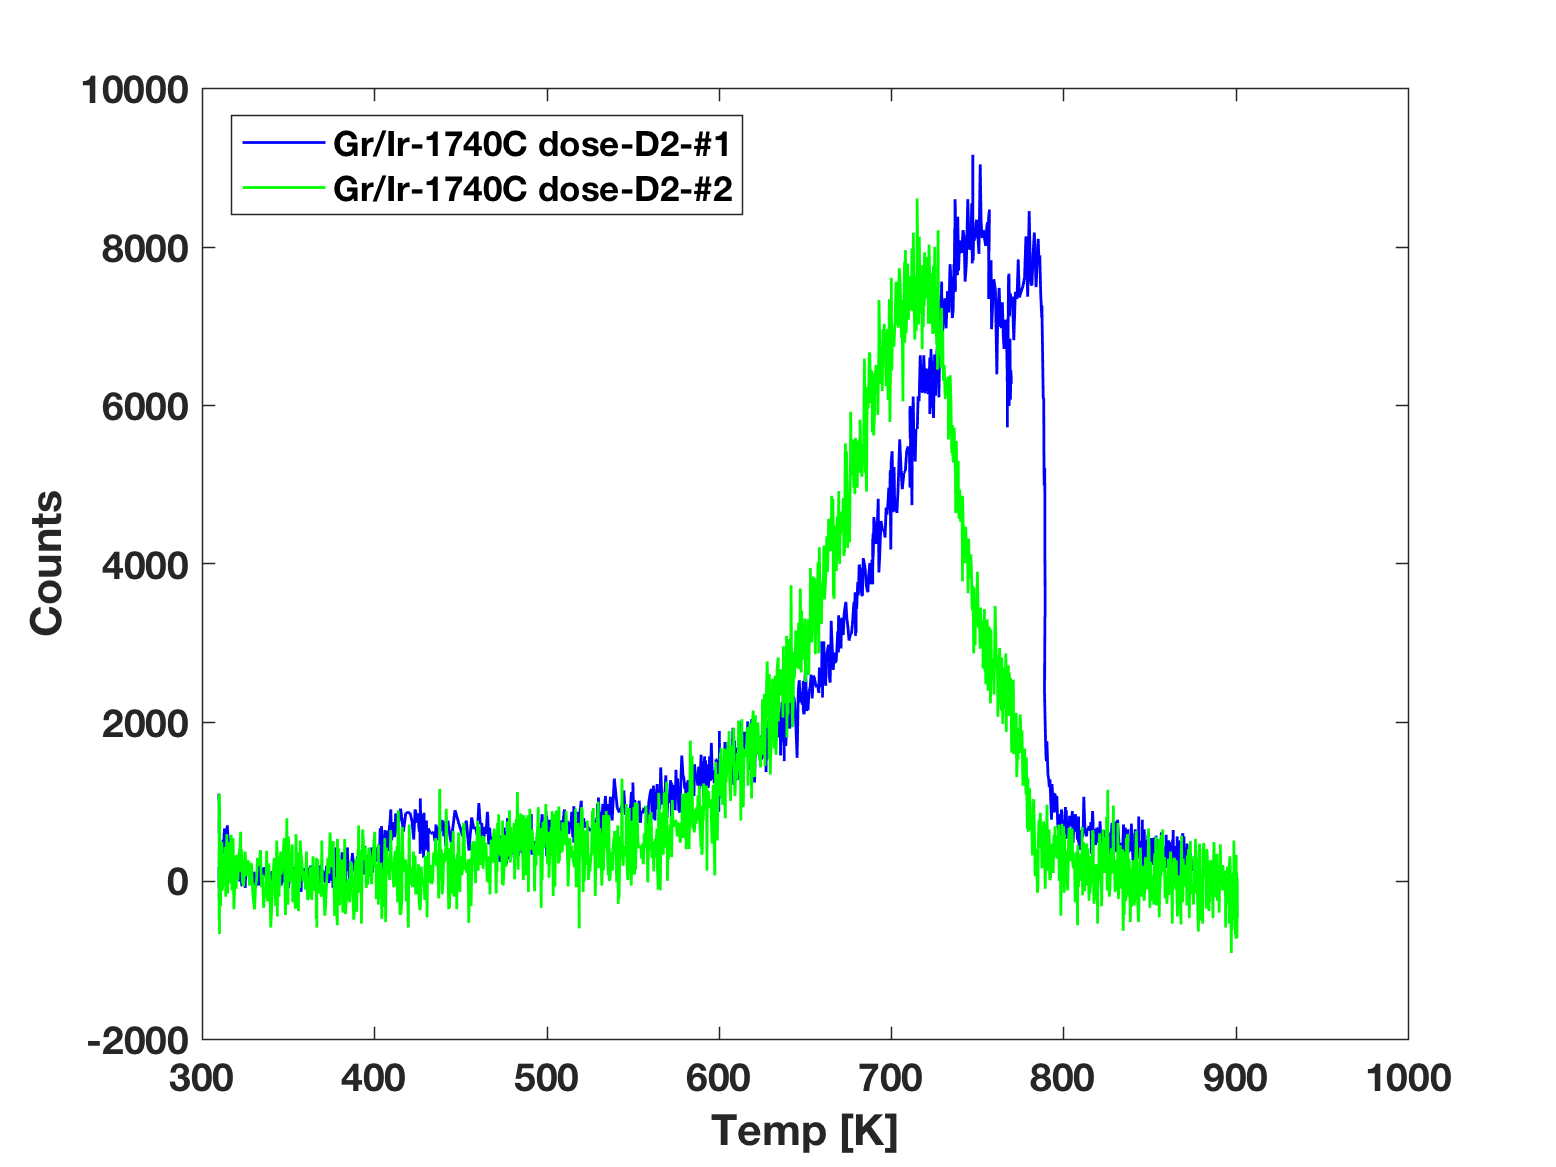
\includegraphics[width=\textwidth]{TPD/050516IrSorenD2dose1hourtemp.png}
    \caption{TPD of Gr/Ir after 1 hour dose of D$_2$ with a doser temperature of 1740 \degree C.}
    \label{TPD:D2}
  \end{subfigure}\hspace{0.5cm}
  \begin{subfigure}[b]{0.45\textwidth}
    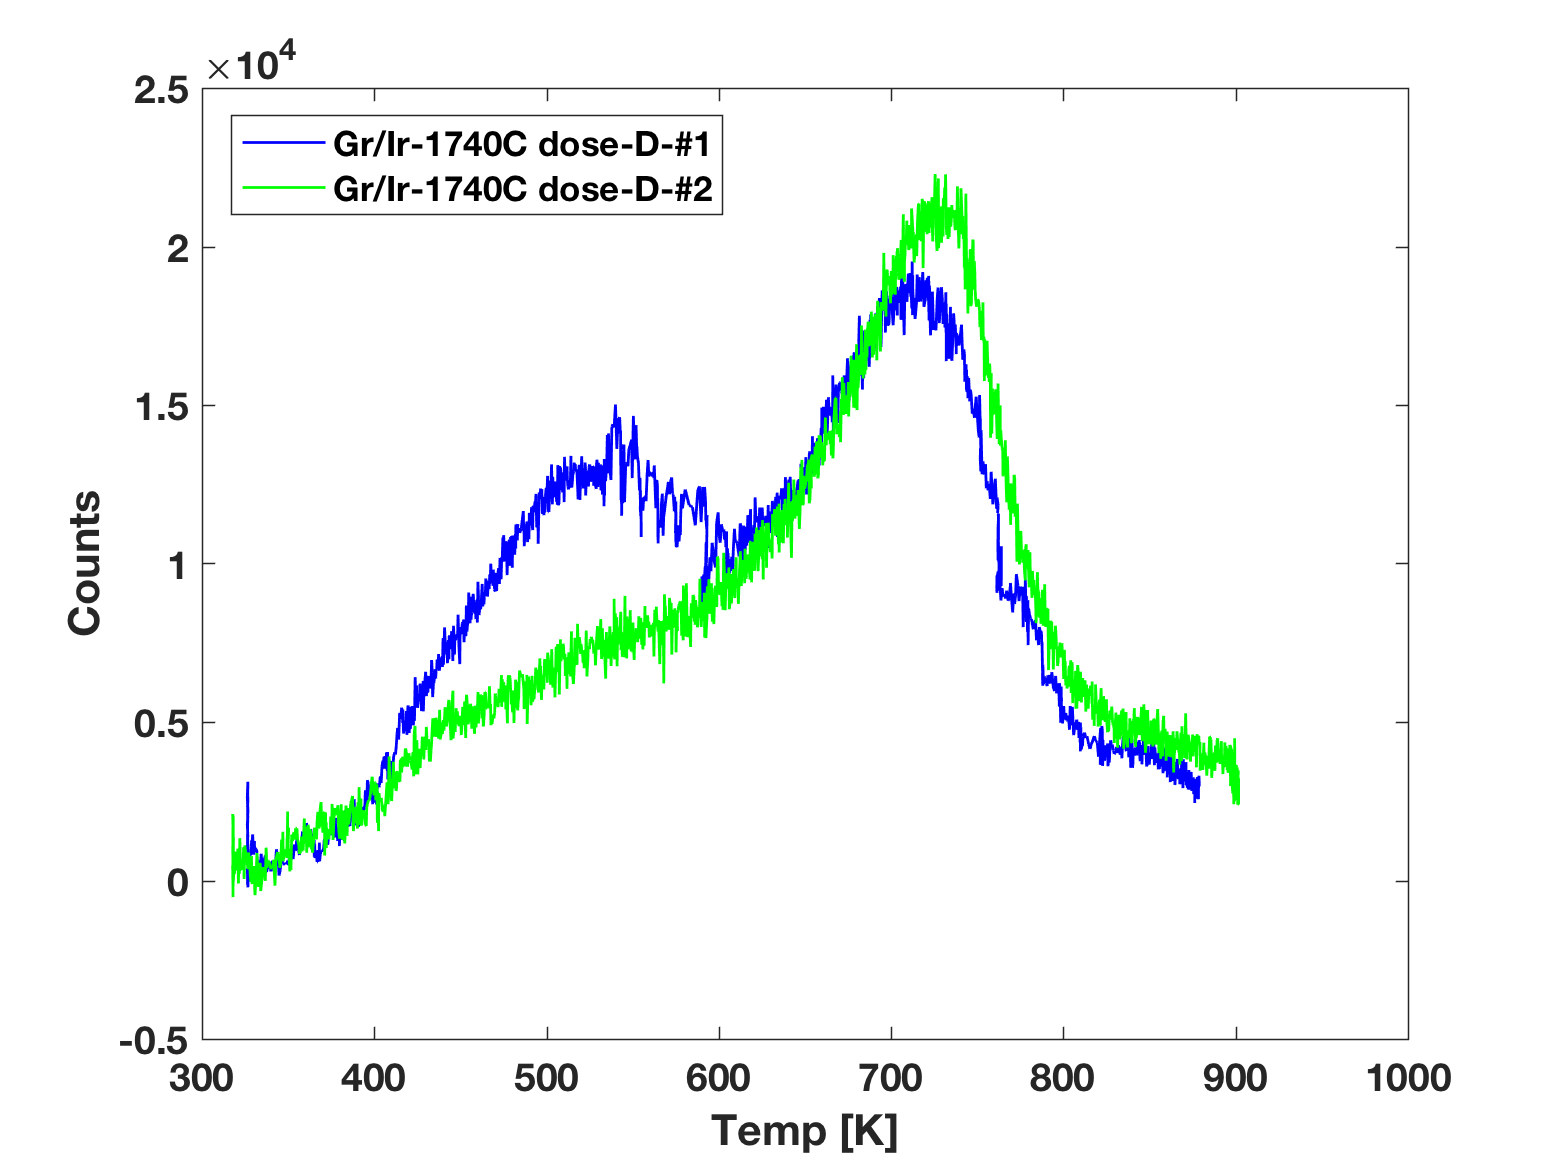
\includegraphics[width=\textwidth]{TPD/050516IrSorenDdose1hourtemp.png}
    \caption{TPD of Gr/Ir after 1 hour dose of atomic deuterium with a doser temperature of 1740 \degree C.}
    \label{TPD:D}
  \end{subfigure}
  \caption{}
  \label{TPD:all}
\end{figure}


\begin{figure}[H]
  \centering
  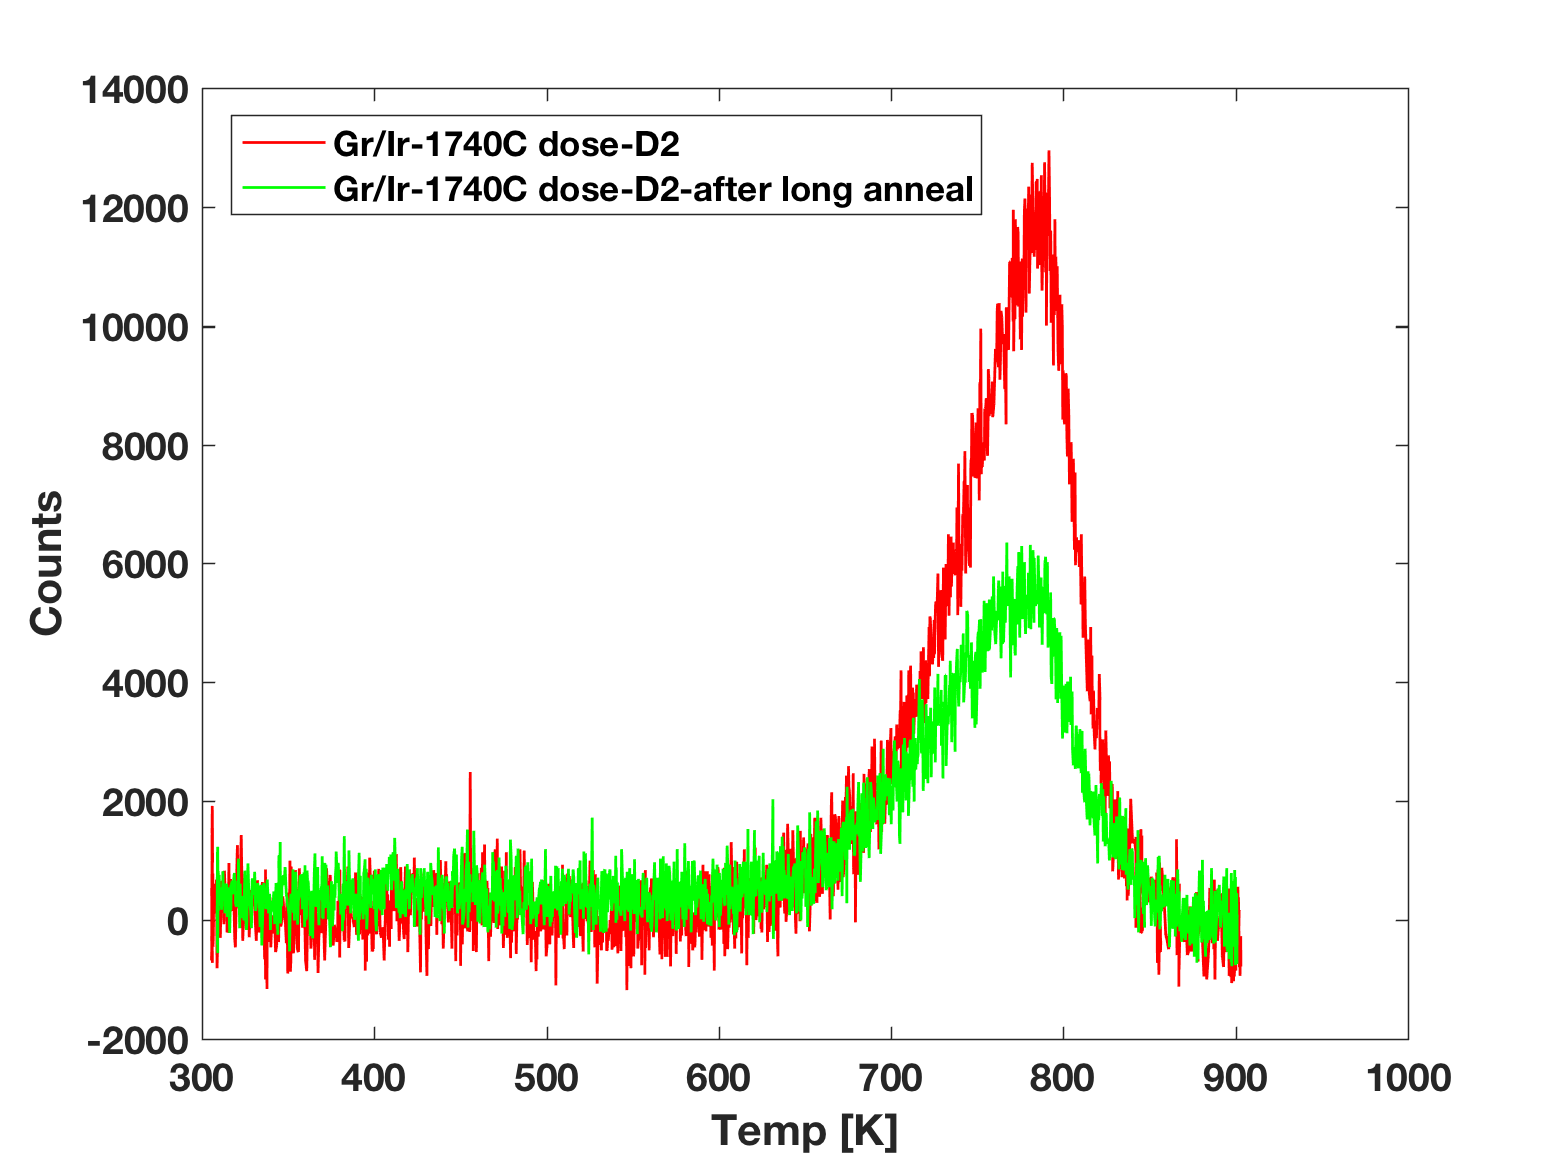
\includegraphics[width=0.6\textwidth]{TPD/GrIr1740CD2longannealtemp.png}
  \caption{}
  \label{TPD:bilayer}
\end{figure}
\section{Bilayered graphene on Ir}


\section{LEED of bilayered sample}

\begin{figure}[H]
\makebox[\textwidth][c]{
  \begin{subfigure}[b]{0.3\paperwidth}
    \includegraphics[height=\textwidth]{LEED/No" "flash/145eV.JPG}
    \caption{LEED without flashing. 145eV}
    \label{}
  \end{subfigure}
  \begin{subfigure}[b]{0.3\paperwidth}
    \includegraphics[height=\textwidth]{LEED/Low" "T" "flash/145eV.JPG}
    \caption{LEED after low temperature flash of the sample. 145eV}
    \label{}
  \end{subfigure}
  \begin{subfigure}[b]{0.3\paperwidth}
    \includegraphics[height=\textwidth]{LEED/post" "1090" "flash/145eV.JPG}
    \caption{LEED after high temperature flash. 145eV}
    \label{}
  \end{subfigure}
}
\caption{}
\label{}
\end{figure}
